\chapter{图上的约束优化}
\label{chap:graph-optimization}

前面两章分别回答了“图上有什么关系”和“怎样检索、分解这些关系”。本章在同一类离散结构上
加入目标与约束，研究怎样作选择。在同一张交通网络上，选最短路线、分配各弧流量、
铺一条最省线的连通网络，会得到不同答案：前者选一条路径，流量给各条弧分配数值，
生成树则选一组边。边旁的数字是长度、容量还是建造成本，必须由问题先指定，
方法的正确性依赖它的用途。

本章按选择对象分六类方法。最短路在端点约束下选路线；距离变换同时求多个位置到目标集的距离；
最大流在容量约束下分配各弧流量；最小生成树在连通约束下选连接边；匹配与指派在互斥约束下
两两配对；标记与划分则为每个顶点选离散标签。每类方法都先说明维护什么可行状态，
再说明哪条递推、交换或上下界证据排除了更好的候选，最后交代代价与失效条件。
涉及一般图时记$n=|V|$、无向边数$m$、有向弧数$a$，默认以邻接表访问并另存边的长度、容量或成本。

\section{基于递推与松弛的最短路方法}

以下加权算法统一在有向图上表述，边长为有限实数；无向边可换成两条同长度反向弧，
因此无向负边来回经过就形成负的闭行走。令$\mathcal P_{s,v}$为$s$到$v$的简单路径集合，
$\mathcal W_{s,v}$为允许重复顶点、边的全部有限行走集合，两个目标分别是
\[
  d_{\mathrm{path}}(s,v)=\min_{P\in\mathcal P_{s,v}}\ell(P),\qquad
  d_{\mathrm{walk}}(s,v)=\inf_{W\in\mathcal W_{s,v}}\ell(W),
\]
空候选集约定为$+\infty$。可达时简单路径只有有限条，最小值存在；行走候选可无限。
标准单源算法求的是$d_{\mathrm{walk}}$：若不存在从$s$可达的负环，真实距离$D(v)$满足
\begin{equation}
  D(s)=0,\qquad
  D(v)=\min_{u\to v}\{D(u)+\ell_{u,v}\}\quad(v\neq s),
  \label{eq:graph-theory-shortest-path-bellman}
\end{equation}
空前驱的最小值取$+\infty$。但这组等式本身不唯一确定距离：
$s\to a$长$5$、$a\leftrightarrow b$两弧长$0$时，任何$D(a)=D(b)\leq5$都满足局部等式，
实际距离却是$5$。所以算法必须从“源为零、其余为无穷”的标签出发，并保存实际路线见证。
下面三种一般方法按可用的结构区分：DAG靠拓扑序一遍完成，Bellman--Ford允许反复修正，
Dijkstra在非负边长下永久确定标签；编辑距离与DTW则是DAG状态递推的两个专门应用。

\subsection{DAG拓扑递推法}

DAG中到达一个顶点的全部前驱都能先算完，标签此后不再被修正。
初始化$L(s)=0$、其余$+\infty$、前驱为空，按一个拓扑序访问$u$，对每条出弧$u\to v$用候选
$L(u)+\ell_{u,v}$松弛：严格更小时更新$L(v)$与$p(v)$。
\begin{algorithm}[DAG拓扑递推最短路]
  先求一个拓扑序；按序处理每个顶点，处理$v$时它的所有入邻居都已处理完毕，
  松弛其全部出弧。终点标签有限时沿前驱逆序恢复路径。
\end{algorithm}
对拓扑序归纳：每条到达$v$的非空路径以某条$u\to v$结束，其前缀成本不小于已求出的$L(u)$，
而每个有限标签又都有实际路径见证，两个方向夹定最小值。
拓扑排序与扫描全部弧共$O(n+a)$，额外$O(n)$。这里允许负边，
因为正确性依赖无环次序，而不依赖“路径前缀比整条路径短”。

在四点DAG（$s\to a$长$2$，$s\to b$长$5$，$a\to b$长$-1$，$a\to t$长$5$，$b\to t$长$2$）上，
按$(s,a,b,t)$：处理$s$得$a=2,b=5$；处理$a$把$b$改为$1$、$t$改为$7$；
处理$b$把$t$改为$3$，恢复路径$s\to a\to b\to t$。

\paragraph{编辑距离的网格递推（扩展）}
同一个“无环状态网格”还可由两条序列的前缀长度构造。令$E(i,j)$为把序列$a$的前$i$个元素
改成序列$b$前$j$个元素所需的最少单元素插入、删除、替换次数。最后一步只有三类：
删$a_i$、插$b_j$、末元素匹配或替换，故
\begin{equation}
  E(0,j)=j,\quad E(i,0)=i,\qquad
  E(i,j)=\min\bigl\{E(i-1,j)+1,\ E(i,j-1)+1,\
    E(i-1,j-1)+\mathbb I_{\{a_i\neq b_j\}}\bigr\}.
  \label{eq:graph-edit-distance-recursion}
\end{equation}
每条状态边都使$i+j$增加，所以这是DAG上的最短路，$E(m,n)$即\term{Levenshtein编辑距离}。
对$(A,B)$与$(A,C,B)$，三行四列分别为$(0,1,2,3)$、$(1,0,1,2)$、$(2,1,1,1)$，
沿“匹配$A$—插入$C$—匹配$B$”得距离$1$。全表连同前驱为$O((m+1)(n+1))$时间与存储，
只求值时用两行可降到$O(n+1)$空间；字符还是词为计数单位须先固定，
相邻交换不设为一次操作，树编辑还需另行规定层级规则，不能展平成字符串套用同一距离。

\paragraph{\term{动态时间规整}（扩展）}
两序列以不同速度经历同一过程时，要让一侧一个读数对应另一侧多个读数。
令局部差异$c(i,j)\geq0$，对齐路径从$(1,1)$到$(m,n)$，每步取$(1,0),(0,1),(1,1)$，则
\begin{equation}
  D(i,j)=c(i,j)+\min\{D(i-1,j),D(i,j-1),D(i-1,j-1)\},\quad D(0,0)=0,
  \label{eq:graph-dtw-recursion}
\end{equation}
正下标的边界行列取$+\infty$，强制两端都参与全局对齐，所以恰一条序列为空时不可行，
不能照搬编辑距离的有限边界。对$a=(1,2)$、$b=(1,1,2)$取绝对值差，
路径$(1,1),(1,2),(2,3)$成本为零；不同长度序列可能零成本，故DTW不自动满足度量公理。
带宽约束$|i-j|\leq w$在$|m-n|>w$时连终点都排除；要最小化平均成本须把路径长度纳入目标，
不能把最小总成本事后除以长度。

\subsection{Bellman--Ford松弛法}

有环时前驱距离可能在以后下降，一遍更新不够。令$L^{(0)}(s)=0$、其余为$+\infty$，
每一轮右侧全部读取上一轮标签：
\[
  L^{(k)}(v)=\min\Bigl\{L^{(k-1)}(v),\
    \min_{u\to v}\bigl(L^{(k-1)}(u)+\ell_{u,v}\bigr)\Bigr\}.
\]
\paragraph{同步松弛的状态与逐轮更新}
\begin{algorithm}[同步Bellman--Ford]
  每轮复制上一轮标签，逐弧用上一轮值计算候选并取最小；重复至多$n-1$轮，
  若一整轮没有任何更新可提前停止。需要路线时连同轮次一起记录前驱。
\end{algorithm}
可归纳证明$L^{(k)}(v)$恰为至多$k$条边到达$v$的最小行走成本：
$k=0$只有源的零步行走，下一轮候选由旧行走或旧前缀加末弧组成。
在上面的四点DAG上逐轮标签为$(0,\infty,\infty,\infty)$、$(0,2,5,\infty)$、
$(0,2,1,7)$、$(0,2,1,3)$。

\paragraph{轮数上界与就地更新}
不受可达负环影响的目标，其行走可删去非负闭合段，最短见证至多$n-1$条边，故$n-1$轮足够。
常用的就地更新在一轮内提前传播新值，此时“恰为至多$k$边最优”的解释只属于同步版本，
但因仍覆盖全部候选且标签都有路线见证，轮数上界不变。

\paragraph{负环种子与后继标记}
完成$n-1$轮后固定标签，再检查所有满足$L(u)<+\infty$且$L(u)+\ell_{u,v}<L(v)$的弧，
把其终点作为种子，并沿出弧遍历种子的全部后继，标为$-\infty$。
正向看，种子有一条比全部至多$n-1$边行走更优的至多$n$边行走，其中必含重复顶点且含负环；
反向看，任一从源可达的负环若环上没有可改善弧，沿环把不等式相加会得到$0\leq\ell(\text{环})<0$的矛盾。
所以标记的恰是“从源可达负环、且该环能继续到达”的目标。
\begin{figure}[!htb]
  \centering
  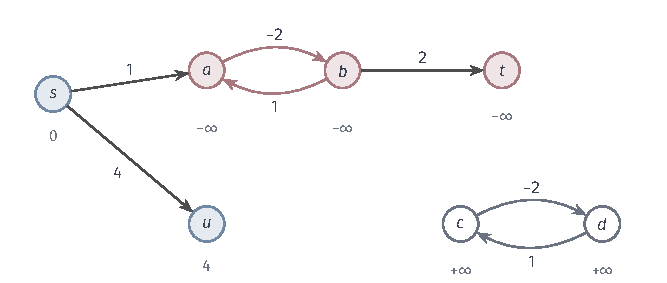
\includegraphics[width=112mm]{figures/01-mathematical-preliminaries-upper/00-shared/tikz/graphs-and-signals-comprehension-additions/graph-negative-cycle-reach.pdf}
  \caption{三种距离状态同处一图。可达负环上的$a,b$及其后继$t$行走下确界为$-\infty$；
  未回接旁支$u$距离有限（$4$）；与$s$不连通的负环$c,d$不影响本次单源查询，距离为$+\infty$。}
  \label{fig:vol1-add-graph-negative-cycle-reach}
\end{figure}
如图~\ref{fig:vol1-add-graph-negative-cycle-reach}，受影响的$-\infty$、
旁支有限距离、不可达$+\infty$要分别报告。同步实现保守时间为$O(n(n+a))$、
状态$O(n)$；若保存全部轮次前驱以回溯有限见证，需$O(n^2)$条记录，
负无穷目标只给负环证据、不可达点无路径。

\subsection{基于贪心选择的Dijkstra法}

若边长全部非负，就能每次永久确定一个顶点，因为到未确定点的更远路线无法靠后半程把成本降下来。
\begin{algorithm}[Dijkstra]
  初始化$D(s)=0$、其余$+\infty$、已确定集为空，把源放入按距离排序的优先队列。
  每次取暂定距离最小的未确定点$u$，永久确定它，再用$D(u)+\ell_{u,v}$松弛其出邻居，
  改善时更新距离、前驱并降键（或重复插入、出队时跳过过期条目）；队列空结束。
\end{algorithm}

\begin{theorem}[Dijkstra算法的贪心正确性]
  \label{thm:graph-theory-dijkstra-correctness}
  若全部边长非负，则顶点$u$被选入已确定集合时，其暂定距离$D(u)$
  等于从$s$到$u$的行走下确界，也等于简单路径最小值。
\end{theorem}
\begin{proof}
有限暂定标签都来自实际路线，故$D(v)\geq D_{\text{真}}(v)$。假设此前确定的点都正确，
考虑新选入的$u$。若有更短路径，取其上第一个未确定点$y$及其已确定前驱$x$，
松弛给出$D(y)\leq D(x)+\ell_{x,y}$，不超过该路径到$y$的前缀；
剩余边长非负使前缀不超过整条路径，而最小键选择又给$D(u)\leq D(y)$，矛盾。
最小键为无穷时尚有可达点也会与“跨出已确定集的第一条边必产生有限标签”矛盾，故这些点确不可达。
\end{proof}
非负性恰用在“前缀代价不超过全路径”这一步。索引二叉堆支持$O(\log n)$取最小与降键，
邻接表下总时间$O((n+a)\log n)$、额外$O(n)$。
在前面的非负四点图上依次确定$a=2$、$b=3$、$t=5$。
反例$s\to a$长$2$、$s\to b$长$5$、$b\to a$长$-4$中没有负环，
算法仍会先把$a$误定为$2$（真实距离$1$），所以条件必须针对机制核验。

\section{基于多源传播与下包络的距离变换方法}

有时要为每个位置求到某个目标集合$F$的距离$D(p)=\min_{q\in F}d(p,q)$（空$F$取$+\infty$）。
先固定$d$是沿邻接行走的路径长度还是直接按坐标差定义的距离；障碍会影响前者而不影响后者。

\subsection{多源BFS传播法}
单位边长时把所有目标位置同时置零、入队，其余为$+\infty$，BFS分层证明原样适用：
首次发现距离就是到任一目标的最少边数，并给一条见证。
在一维位置$0$至$4$、目标$\{0,4\}$上，初始队列$[0,4]$，逐层得到距离$(0,1,2,1,0)$。
非负加权边改用多源Dijkstra（所有源同时为零），不能用FIFO首次发现就定值。
一般邻接表为$O(n+m)$，$P$个位置的规则网格为$O(P)$。

\subsection{双向扫描法}
无障碍矩形的4邻接距离可两遍扫描：正向（上到下、左到右）用上、左邻居加一取小，
反向用下、右邻居加一取小。任一源—终点的曼哈顿最短路都可在矩形内选一个转折点，
拼成一段右/下步加一段左/上坡，故两遍已覆盖最优见证、不会低估，总时间$O(P)$；
有障碍时路线可能多次换向，该保证失效。
轴向步成本$a$、对角步成本$b$，在$0<a\leq b\leq2a$且无障碍时，
最短成本为$b\min(|\Delta i|,|\Delta j|)+a\bigl||\Delta i|-|\Delta j|\bigr|$。
取$a=3,b=4$得常用\term{倒角距离}，归一化后对角为$4/3$而非$\sqrt2$，
所以它是该图上的精确路径距离，却不是精确欧氏距离。

\subsection{一维二次下包络法}
\label{sec:graph-quadratic-distance}
要精确计算平方欧氏距离，可把目标写成$q\in F$时$f(q)=0$、其余$+\infty$，
再最小化$f(q)+a(x-q)^2$。先研究一维问题
\begin{equation}
  \mathcal D(x)=\min_{q=0,\ldots,n-1}\{f(q)+a(x-q)^2\},\qquad a>0,
  \label{eq:graph-quadratic-distance-transform}
\end{equation}
其中$f$也可取任意有限实数（此时结果可能为负，不必是距离）。
直接枚举需$O(n^2)$，但所有候选是曲率相同的抛物线，只需保留某处可能最低者。
对中心$p<q$，消去共同的$ax^2$项，两曲线唯一交点为
\begin{equation}
  s(p,q)=\frac{f(q)+aq^2-f(p)-ap^2}{2a(q-p)}.
  \label{eq:graph-parabola-intersection}
\end{equation}
交点右侧较大中心$q$更低，故随输出坐标增大，最低候选的中心只向右移。
\begin{algorithm}[抛物线下包络]
  维护候选中心栈$v_0,\ldots,v_k$及各自开始占优的位置
  $z_0=-\infty<z_1<\cdots<z_k$，以$+\infty$收尾。跳过全部$f$为无穷的候选；
  新中心$q$入栈前求它与栈顶的交点$s$，若$s\leq z_k$说明旧栈顶已被全面压低，弹出后重算，
  直到$s>z_k$再压入。建栈后用只向右移动的指针按整数$x$选覆盖当前位置的候选求值。
\end{algorithm}
每个中心至多入栈、出栈一次，查询指针只前进，总时间与存储均为$O(n)$。
$f(0)=f(4)=0$、其余无穷时两抛物线交于$2$，输出$(0,1,4,1,0)$；
加入$f(1)=10$的短例可看到中间候选被弹出，结果与逐候选取最小一致。

\subsection{逐轴二次距离变换法}
二维（及高维）二次成本各轴项不混合，可逐层换序：
\[
  \min_{q_1,q_2}\{f(q_1,q_2)+a_1(p_1-q_1)^2+a_2(p_2-q_2)^2\}
  =\min_{q_2}\Bigl\{a_2(p_2-q_2)^2+
    \min_{q_1}[f(q_1,q_2)+a_1(p_1-q_1)^2]\Bigr\}.
\]
先沿第一轴对每条直线跑一维变换，中间数组再沿第二轴跑，$d$维$P$个位置共$O(dP)$；
保存最近源时要把前一轴的源索引带到后一轴。$a_j=1$且$f$为零/无穷指标时输出平方欧氏距离，
最后逐点开方才是欧氏距离：$\{0,4\}$的平方输出$(0,1,4,1,0)$开方为$(0,1,2,1,0)$。
最大化“响应减二次惩罚”时令$f=-R$再取反；线性位移项可分别并入输入与输出，
但含两轴混合乘积的成本一般不能逐轴分离。

\section{基于残量增广的最大流方法}

这次不是选一条路线，而是在多条路线可并行、每条弧又有通过上限时共同分配流量。
两条共用容量$1$的首弧的路线合计至多送$1$，不能各送$1$。
固定有限有向网络与不同端点$s,t$，每条弧有有限非负容量$c_{i,j}$，
非弧按容量$0$延拓（这些零条目不是新通道）。一个\term{流}（flow）$f$满足
\[
  0\leq f_{i,j}\leq c_{i,j},\qquad
  \sum_{u:u\to v}f_{u,v}=\sum_{w:v\to w}f_{v,w}\quad(v\neq s,t),
\]
即容量约束加内部流守恒。流值$|f|$是源净流出；对内部守恒式求和可知它等于汇净流入，
不是全图弧流量之和。取$s\in S,t\notin S$，割容量为
$c(S,V\setminus S)=\sum_{i\in S,j\notin S}c_{i,j}$，只计源侧跨向汇侧的容量。
对$S$内部守恒求和可知任意流值不超过任意割容量。

\subsection{残量增广法}
已选路线可能抢占更好安排，所以要能撤回。对每条原弧$i\to j$建立容量$c_{i,j}-f_{i,j}$的正向残量弧
（可追加）和容量$f_{i,j}$的反向残量弧（可撤回），只保留正容量残量弧，并保留原弧身份；
撤回不要求原网络真有$b\to a$通道。原弧容量$3$、已发$2$时，正向残量$1$、反向残量$2$。

\begin{algorithm}[残量增广最大流]
  从零流开始；在当前残量网络搜索$s$到$t$的路径，没有则停止；
  取路径上最小残量$\delta$为瓶颈，沿正向残量把对应原流加$\delta$、沿反向残量减$\delta$；
  更新残量后重复，结束时输出流以及残量网络中从$s$可达的集合$S$。
\end{algorithm}
瓶颈保证不超容量、不为负，路径内部流入流出变化抵消，源净流出严格增加$\delta$。

\begin{theorem}[最大流最小割定理]
  \label{thm:graph-theory-max-flow-min-cut}
  在有限非负容量网络中，最大$s$--$t$流值等于最小$s$--$t$割容量。
\end{theorem}
\begin{proof}
可行流由有限个闭有界线性约束定义、含零流，故最大流$f$存在。若其残量网络还有$s$--$t$路径，
按上法增广得到更大流，矛盾。取残量网络中$s$的可达集$S$，则跨出$S$的原弧必已满流
（否则可沿正向残量离开），从外面流入$S$的原弧必为零流（否则可沿反向残量离开），
于是$|f|$恰等于割容量$c(S,V\setminus S)$。任意流不超过任意割，故此流与此割分别最优。
\end{proof}

\begin{figure}[htbp]
  \centering
  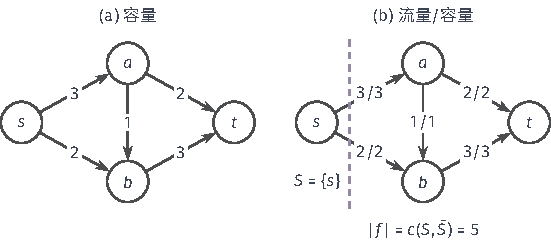
\includegraphics[width=93.282mm]{figures/01-mathematical-preliminaries-upper/07-graphs/tikz/graph-theory-flow-cut-certificate/figure.pdf}
  \caption{同值流与割构成最优性证书。跨出$S=\{s\}$的容量为$3+2=5$，等于实现的流值；
  图中画原网络弧，不画残量反向弧。}
  \label{fig:graph-theory-flow-cut-certificate}
\end{figure}

整数容量下从零流每次增广整数瓶颈，流始终为整数、每次至少增$1$，
源出容量和$C_s$有限，故至多$C_s$次增广终止，也证明了整数最优流存在；
这个次数依赖容量数值，不是位长多项式。容量取$3,2,1,2,3$时
依次沿$s\to a\to t$、$s\to b\to t$、$s\to a\to b\to t$增广$2,2,1$得流值$5$，
割$\{s\}$容量也是$5$（图~\ref{fig:graph-theory-flow-cut-certificate}）。
单位容量网还能演示撤回：首次沿$s\to a\to b\to t$后，第二次借残量$b\to a$改道，
最终真实路线为$s\to a\to t$与$s\to b\to t$。线性搜索残量路的基本实现时间为
$O((C_s+1)(n+a))$；任意实容量下紧性保证最优流存在，却不保证任意选路有限终止。

\section{基于安全选边的最小生成树方法}
\label{sec:graph-theory-minimum-spanning-tree}

每条无向边附带建造成本时，要在覆盖全部顶点、连通且无环的边集中选总成本最小者，
即\term{最小生成树}（minimum spanning tree, MST）。它最小化的是连接全网的建造费用，
不保证树上距离等于原图最短路：三角形边长$2,2,3$时MST费用$4$，原长$3$直连的两点在树上距离变为$4$。

对非平凡割$(S,V\setminus S)$，跨割成本最小的边称轻边。
\begin{lemma}[最小生成树的割性质]
  \label{lem:graph-theory-mst-cut-property}
  若边集$A$已包含在某棵MST中，且某割不切断$A$的任何边，则该割的一条轻边$e$
  可与$A$一起包含在某棵MST中。
\end{lemma}
\begin{proof}
取包含$A$的MST $T$。若$e\notin T$，加入$e$形成唯一环，环上必有另一条跨割边$f$才能回到原侧；
轻边给$w_e\leq w_f$，删$f$得到的生成树$T+e-f$成本不增，且因割未切$A$而$f\notin A$，
新树仍含$A$与$e$。
\end{proof}
负成本不影响这个相对比较；平局可产生多棵MST，但最小总成本唯一。

\subsection{Kruskal分量合并法}
\begin{algorithm}[Kruskal]
  先为每个顶点建单元并查集类，把全部边按成本（并列时按固定边序）排序；
  逐条取边$(u,v)$，若find代表相同则跳过（加入会成环），否则选中该边并union两类、分量数减一；
  连通图选满$n-1$条即停止，否则输出最小生成森林并报告不连通。
\end{algorithm}
在五点七边图（$ab=1,bc=2,cd=3,ac=4,bd=5,ce=6,de=7$）上，
依次接纳$ab,bc,cd$（此时$\{a,b,c,d\}$与$\{e\}$两类，累计$6$），
$ac$、$bd$因成环跳过，接纳$ce$后全连通，所选边为$\{ab,bc,cd,ce\}$，成本$12$。
接纳边之所以安全，是因为取其一端当前分量作割时，所有更轻边都已处理、不可能还跨此割，
当前边正是轻边。排序$O(m\log m)$，并查集在路径压缩加按秩合并下摊还$O(m\alpha(n))$。

\subsection{Prim单树扩展法}
\begin{algorithm}[Prim]
  固定起点$a$，维护一个已连通集$S$，为每个外部点$v$保存键
  $\operatorname{key}(v)=\min_{u\in S}w_{u,v}$及对应父点；
  反复取键最小的未加入点$u$加入$S$、把其父边收入树，并用$u$的邻边松弛外部点的键（用索引堆降键），
  直到$S$覆盖该分量。
\end{algorithm}
键是一条跨割边的成本，不是Dijkstra的累计路线长度。
在同一五点图上从$a$开始：先取$ab$（键$1$），$b$把$c$的键从$4$改为$2$、$d$设为$5$；
取$bc$后$d$改为$3$、$e$设为$6$；取$cd$后检查$de=7$不优于$e$的$6$；最后取$ce$，
得到同样四条边、成本$12$。每次最小键恰是割$(S,V\setminus S)$的轻边，割性质逐步保证可扩成MST。
索引堆下$O((n+m)\log n)$，朴素数组选最小为$O(n^2+m)$。
从$e$出发会先取$ec=6$再取$cb=2,ba=1,cd=3$，说明Prim的选边成本不必递增，
与Kruskal全局排序的思想不同；非连通图逐分量求森林。
另外，第~\ref{chap:graph-traversal}章团树构造在团候选图上求最大总交集权，把比较改为取最大即可复用同一交换机制，
但其运行交集保证来自团树定理，不是贪心本身给出的。

\section{基于交替增广的匹配与指派方法}

二部图$\mathcal G=(U,W,E)$的\term{匹配}（matching）是一组不共享端点的边。
不能再加边的称极大匹配，边数最多的才称最大匹配——局部加不进边，
仍可能靠替换已有边扩大配对。先最大化配对数量，再在“每个左对象都必须配对”的要求下最小化成本。

\subsection{交替路径增广匹配法}
建一个网络：源到每个$u\in U$连容量$1$弧，每条候选边改容量$1$弧$u\to w$，
每个$w\in W$再连容量$1$弧到汇。任一匹配对应一个同值整数流；
源、汇两侧的单位容量保证每个左右点至多选一次，故整数最大流的值恰为最大匹配的边数，
不能用分数阈值化代替实际配对。
匹配的\term{增广路径}两端都是未匹配点，路径上未选边与已选边交替出现；
沿路径翻转后内部点仍各有一条匹配边，两端各添一条，匹配数增加$1$。
它正是该单位容量网络的残量$s$--$t$路径：未匹配边正向走、已匹配边反向撤回。
如图~\ref{fig:graph-theory-matching-augmentation}，已有$\{a-x,b-y\}$时，
自由点$c$沿$c-y-b-z$搜索，撤$b-y$、加$c-y$与$b-z$，得到大小$3$的匹配。
无增广路径即无残量路径，由最大流最小割得最大性证书。
\begin{figure}[htbp]
  \centering
  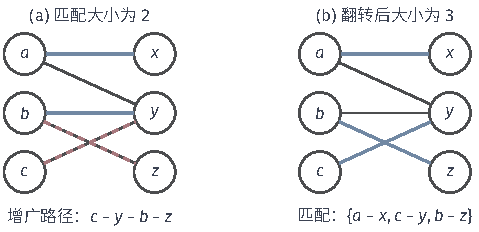
\includegraphics[width=81.188mm]{figures/01-mathematical-preliminaries-upper/07-graphs/tikz/graph-theory-matching-augmentation/figure.pdf}
  \caption{沿交替路径$c-y-b-z$重排匹配：撤去$b-y$，加入$c-y,b-z$，保留$a-x$，
  配对数由$2$增为$3$。连线表示候选配对，不表示因果方向。}
  \label{fig:graph-theory-matching-augmentation}
\end{figure}
一般含奇环的非二部图不能用这套左右流构造；加权匹配目标也不同，需另建机制。

\subsection{匈牙利\term{紧边}增广法}
\label{sec:graph-weighted-assignment}
设左侧$m$个对象都须分到右侧$n\geq m$个不同对象，允许边成本为有限实数$c_{ij}$，
\begin{equation}
  \min_x\sum_{i,j}c_{ij}x_{ij},\qquad
  \sum_jx_{ij}=1,\quad \sum_ix_{ij}\leq1,\quad x_{ij}\in\{0,1\}.
  \label{eq:graph-rectangular-assignment}
\end{equation}
补$n-m$个零成本虚拟左对象可化为$N=n$阶方阵完整指派（每行每列恰选一条），虚拟对象只占用未用列。
若允许真实对象不匹配，不能只把等式改成不等式（非负成本下空匹配会最优），
而要为每个左对象设成本$\rho_i$的专属虚拟列、每个右对象设成本$\eta_j$的专属虚拟行，
非专属真实—虚拟配对禁配，使总成本恰为配对成本加未匹配惩罚。

给每行、每列选\term{指派势}$u_i,v_j$，使每条允许边满足
\begin{equation}
  u_i+v_j\leq c_{ij};
  \label{eq:graph-assignment-potentials}
\end{equation}
任何完整指派的成本都不小于$\sum_i u_i+\sum_j v_j$（每行每列恰计一次）。
取等号的边称紧边；若能只用紧边完成完整指派，其成本恰等于该下界，即全局最优，
这同时证明对应的线性松弛有整数最优解。
\begin{algorithm}[匈牙利紧边增广]
  取$u_i=\min_j c_{ij}$、$v_j=0$建初始可行势；维护紧边匹配，反复从一个自由行出发
  沿“紧的未匹配边到列、已匹配列沿其匹配边回行”建交替树。到达自由列就翻转增广；
  若树被卡住，令$S,T$为树中行、列，取$\delta=\min_{i\in S,j\notin T}(c_{ij}-u_i-v_j)$，
  把$S$中行势加$\delta$、$T$中列势减$\delta$，保留可行性与已有紧匹配并至少新增一条紧边，
  再继续，直到全部行匹配。
\end{algorithm}
对成本矩阵$\begin{bmatrix}1&2\\1&100\end{bmatrix}$，逐行贪心得$101$；
初始势$u=(1,1),v=(0,0)$，从第二行建树得$\delta=1$，调势至$u=(2,2),v=(-1,0)$后
第一行第二列变紧，翻转得总成本$3$，恰等于势下界$2+2-1=3$。
稠密实现为每个未入树列维护最小剩余成本及前驱，每次增广$O(N^2)$、至多$N$次，共$O(N^3)$、
额外$O(N)$；这是实数算术操作数，有限精度时要另设相等容差。

\section{基于图割与谱松弛的标记和划分方法}

令顶点标签$z_i\in\{0,1\}$，一元成本$D_i(z_i)$表示该点自身偏好，
成对成本$\theta_{i,j}(z_i,z_j)$表示相邻标签相容性，目标为
\begin{equation}
  \mathcal E(\bm z)=\sum_iD_i(z_i)+\sum_{\{i,j\}\in E}\theta_{i,j}(z_i,z_j).
  \label{eq:graph-theory-binary-pairwise-energy}
\end{equation}
二值时平方差等于绝对差，非负边差可由跨割边支付，但任意四项成对成本未必有这种表示。
先给出离散优化常用的证书思路：扩大可行域得到的松弛最优值是原离散最优值$\mathcal E^\star$的下界$L$；
把连续解恢复成可行离散配置并算出其原目标值$U$，则
$0\leq U-\mathcal E^\star\leq U-L$，$U-L$只是次优差距的上界，只有下界紧时才等于真实误差。

\subsection{二值\term{次模}图割法}
若一条边的四项成本满足次模条件
\begin{equation}
  \theta_{i,j}(0,0)+\theta_{i,j}(1,1)
  \leq\theta_{i,j}(0,1)+\theta_{i,j}(1,0),
  \label{eq:graph-theory-pairwise-submodularity}
\end{equation}
就可以把成对项改写成“常数＋线性项＋非负边差”。令
\begin{align}
  w_{i,j}&=\frac{\theta_{0,1}+\theta_{1,0}-\theta_{0,0}-\theta_{1,1}}2,
    \label{eq:graph-theory-cut-pair-weight}\\
  \alpha_i&=\theta_{1,0}-\theta_{0,0}-w_{i,j},\qquad
    \alpha_j=\theta_{0,1}-\theta_{0,0}-w_{i,j},
    \label{eq:graph-theory-cut-unary-shifts}
\end{align}
次模性恰保证$w_{i,j}\geq0$，并可逐代入四种配置验证
\begin{equation}
  \theta_{i,j}(z_i,z_j)=\theta_{0,0}+\alpha_i z_i+\alpha_j z_j+w_{i,j}|z_i-z_j|.
  \label{eq:graph-theory-pairwise-cut-decomposition}
\end{equation}
对所有边累加常数、把线性项并入一元函数，再减去每点两标签成本的最小值使新一元非负，
得到只差一个统一常数的目标。

\begin{theorem}[二值次模成对能量的割表示]
  \label{thm:graph-theory-submodular-cut-representation}
  当一元项与成对项均为有限实数、且每个成对项次模时，存在非负容量的$s$--$t$网络，
  使每个二值配置的割容量等于其能量加同一常数，因而一次最小割给出全局最优配置。
\end{theorem}
\begin{proof}
规定源侧标签为$0$、汇侧为$1$。建弧$s\to i$容量$\widetilde D_i(1)$、$i\to t$容量$\widetilde D_i(0)$：
点$i$在源侧时割断$i\to t$、付$\widetilde D_i(0)$，在汇侧时割断$s\to i$、付$\widetilde D_i(1)$。
每条成对边建两条容量$w_{i,j}$的反向弧，同侧不计、异侧只有源侧到汇侧一条跨割，恰付一次$w_{i,j}$。
于是割容量恰为能量减去统一常数；配置与割两侧归属一一对应，最小割即最优配置。
\end{proof}
\begin{figure}[htbp]
  \centering
  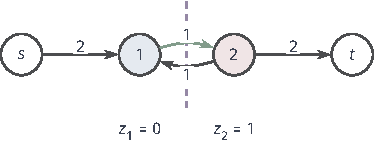
\includegraphics[width=63.281mm]{figures/01-mathematical-preliminaries-upper/07-graphs/tikz/graph-theory-binary-energy-cut/figure.pdf}
  \caption{两变量能量的割表示。点$1$在源侧、点$2$在汇侧时标签为$(0,1)$，
  两条容量$1$的反向弧中只计源侧到汇侧一条，终端弧按所在侧支付。}
  \label{fig:graph-theory-binary-energy-cut}
\end{figure}
例如$D_1=(0,2),D_2=(2,0),w_{12}=1$，四个配置能量为$2,1,5,2$，
最小割恢复$(0,1)$（图~\ref{fig:graph-theory-binary-energy-cut}）。
次模失败时$w_{i,j}<0$，不能用非负容量构造；多标签、高阶或一般非次模目标也不能自动化成一次最小割，
但特殊结构（如链）仍可能用动态规划精确求解。构造网络为$O(n+m)$，总时间还要加上所选最大流的代价。

\subsection{RatioCut谱松弛法}
\label{sec:graph-theory-ratio-cut}
以下设$n\geq2$以便分成两个非空组。单纯最小化跨组边权可能孤立一个弱连点，允许空组时零割更会直接最优。
对指示向量$\bm s=\mathbb I\{i\in S\}$，由第~\ref{chap:graph-objects}章能量式有
\begin{equation}
  \bm s^\top\bm L\bm s=\operatorname{cut}(S,\bar S),
  \label{eq:graph-theory-indicator-cut-energy}
\end{equation}
令$a=|S|>0,b=|\bar S|>0$，\term{比率割}定义为
\begin{equation}
  \operatorname{RatioCut}(S,\bar S)=\operatorname{cut}(S,\bar S)\left(\frac1a+\frac1b\right).
  \label{eq:graph-theory-ratio-cut}
\end{equation}
构造两水平向量（$S$中取$\sqrt{b/a}$、补集中取$-\sqrt{a/b}$），
\begin{equation}
  f_i=\sqrt{b/a}\ (i\in S),\qquad f_i=-\sqrt{a/b}\ (i\notin S),
  \label{eq:graph-theory-ratio-cut-balanced-vector}
\end{equation}
可直接核对$\bm1^\top\bm f=0$、$\bm f^\top\bm f=n$，且
\begin{equation}
  \bm f^\top\bm L\bm f=n\,\operatorname{RatioCut}(S,\bar S).
  \label{eq:graph-theory-ratio-cut-energy}
\end{equation}
去掉“只能取两个水平值”的限制、保留零均值与范数$n$，得到连续松弛
\begin{equation}
  \min_{\bm f^\top\bm1=0,\ \bm f^\top\bm f=n}\frac1n\bm f^\top\bm L\bm f.
  \label{eq:graph-theory-ratio-cut-relaxation}
\end{equation}
在与常量$\bm u_1=\bm1/\sqrt n$正交的子空间谱展开，Rayleigh商是$\lambda_2,\ldots,\lambda_n$的
加权平均，故不小于第二特征值$\lambda_2$，$\sqrt n\,\bm u_2$达到下界；
正权支撑连通时$\lambda_2>0$，$\bm u_2$称费德勒向量。
\begin{algorithm}[谱划分与恢复]
  建立正权支撑上的$\bm L$，求满足常量正交的第二特征方向；把坐标排序，
  在相邻不同值之间设候选阈值（相同坐标整体移动），得到两个非空组；
  逐个按原RatioCut评价，取最好的可行划分并输出其上界$U$，与有效下界$L=\lambda_2$组成证书。
\end{algorithm}
恢复时每移入一个顶点，把连向已在$S$点的边权从割中扣除、连向补集点的加上，
排序加扫描为$O(n\log n+m)$。稠密完整特征分解基准为$O(n^3)$时间、$O(n^2)$存储，
稀疏迭代的代价取决于求解器与谱间隔，不能只因$\bm L$稀疏就断言整体线性。

\subsection{NCut谱松弛法}
改用各组连接权重总量（体积）$\operatorname{vol}(S)=\sum_{i\in S}d_i^{(w)}$衡量平衡，
令$p=\operatorname{vol}(S)>0,q=\operatorname{vol}(\bar S)>0$，定义
\begin{equation}
  \operatorname{NCut}(S,\bar S)=\operatorname{cut}(S,\bar S)\left(\frac1p+\frac1q\right),
  \label{eq:graph-theory-normalized-cut}
\end{equation}
同样的两水平构造（以体积代替点数）给出$\bm y^\top\bm D\bm1=0$、
$\bm y^\top\bm D\bm y=p+q$，且$\bm y^\top\bm L\bm y=\operatorname{vol}(V)\operatorname{NCut}$。
放宽后是度加权Rayleigh问题
\begin{equation}
  \min_{\bm y\neq\bm0,\ \bm y^\top\bm D\bm1=0}
    \frac{\bm y^\top\bm L\bm y}{\bm y^\top\bm D\bm y},
  \label{eq:graph-theory-normalized-cut-relaxation}
\end{equation}
引入尺度与平衡乘子并对$\bm y$求导，左乘$\bm1^\top$用$\bm1^\top\bm L=\bm0$与平衡条件消去乘子，得
\begin{equation}
  \bm L\bm y=\lambda\bm D\bm y,\qquad \bm y^\top\bm D\bm1=0.
  \label{eq:graph-theory-normalized-cut-generalized-eigenproblem}
\end{equation}
作坐标变换$\bm x=\bm D^{1/2}\bm y$，它等价于在$\bm x\perp\bm D^{1/2}\bm1$下
求$\bm L_{\mathrm{sym}}$的第二特征向量，再变回$\bm y=\bm D^{-1/2}\bm x$；
不能把任意驻点当成最小值，也不能在一般不规则图上用组合拉普拉斯的费德勒向量替代，
只有正度正则图$\bm D=d\bm I$时方向相同、特征值缩放$1/d$。零度点体积为零要先分类处理：
若正权支撑有多个正体积分量，可直接按分量分成两个非空正体积组，得NCut为$0$。

\begin{figure}[htbp]
  \centering
  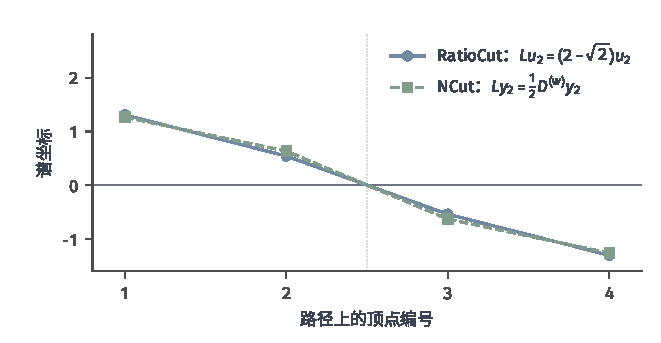
\includegraphics[width=112.0mm]{figures/01-mathematical-preliminaries-upper/07-graphs/matplotlib/graph-theory-spectral-coordinates/figure.pdf}
  \caption{单位权四点路径的两种谱方向：组合拉普拉斯第二特征向量（蓝实线）
  与度加权广义特征向量（绿虚线），二者零阈值都恢复中间分割，但相对幅度不同。}
  \label{fig:graph-theory-spectral-coordinates}
\end{figure}
在四点单位权路径$1-2-3-4$（$\bm D=\operatorname{diag}(1,2,2,1)$）上，
中间分割$\{1,2\}|\{3,4\}$的RatioCut为$1$、两水平商为$4/4=1$，
而组合$\bm L$第二特征值为$2-\sqrt2\approx0.586$、方向正比
$(1+\sqrt2,1,-1,-1-\sqrt2)$（图~\ref{fig:graph-theory-spectral-coordinates}）；
枚举七个非空二分可知离散最优RatioCut为$1$，与松弛下界并不相等。
同一分割两侧体积均为$3$，NCut为$2/3$、加权商$4/6=2/3$，广义第二特征值为$1/2$、
方向正比$(1,\tfrac12,-\tfrac12,-1)$。两法在此例恰好同分组，但方程、向量、下界均不同。
恢复后必须检查两组非空（NCut还要正体积）、重算原离散目标；
特征方向的稳定性还依赖相邻特征值间隔，重根时应考察整个子空间。

\section{本章小结}

\paragraph{按选择对象核对方法}
路径法选一条从源到目标的路线，距离变换同时处理多个位置查询，
流量法共同分配弧容量，生成树法选连接边集，匹配与指派选互不抢占的配对，
标记划分法为每个顶点选配置。同一张图、同一组数字不能省去任务定义。

\paragraph{按状态与证书理解执行}
DAG递推、Bellman--Ford和Dijkstra共享松弛动作，却分别依靠拓扑先后、
重复修正与非负边长下的永久确定；不可达$+\infty$、有限距离与负环影响的$-\infty$要分开输出。
残量增广靠撤回旧流、Kruskal靠分量防环、Prim靠跨割单边键扩树、
匹配与指派靠交替路径替换旧配对，最优性分别由流割同值、割交换或紧边势下界证书保证。

\paragraph{精确图割与谱松弛的边界}
二值次模图割在声明的有限成本条件下给出与原离散目标等价的非负容量构造；
RatioCut和NCut的特征方向只解各自的连续松弛，恢复后要检查非空或正体积、
重算原目标并用有效下界评价次优差距，两种谱方法的坐标、平衡范数与下界不能互换。
代价分析要同时计图表示、候选规模、轮数、队列或表的状态与数值精度。
下一章保持图与函数输入不变，研究顶点函数的谱坐标、滤波扩散、标记细化与配置表汇总。
